\documentclass[8pt, twosided, a4paper]{article}
% 8 point font, A4-sized paper

\usepackage[margin=2.5cm]{geometry}
\usepackage[utf8]{inputenc}

\usepackage[scaled]{helvet}
\renewcommand\familydefault{\sfdefault} 
\usepackage[T1]{fontenc}

\usepackage{pdfpages}
\usepackage{subfiles}
\usepackage{setspace}
\usepackage{multicol}
\usepackage{multirow}
\usepackage{mathtools}

\usepackage{cancel}

\usepackage[inline]{asymptote}

\usepackage{array}
\usepackage{enumitem}
\usepackage{float}
\usepackage{amsfonts}
\usepackage{tikz}
\usetikzlibrary{matrix,fit}
\usepackage{blkarray}
\usepackage{caption}

\begin{document}
\pagenumbering{gobble}

% I did this because it was too dense without it
\setlength{\parskip}{1em}

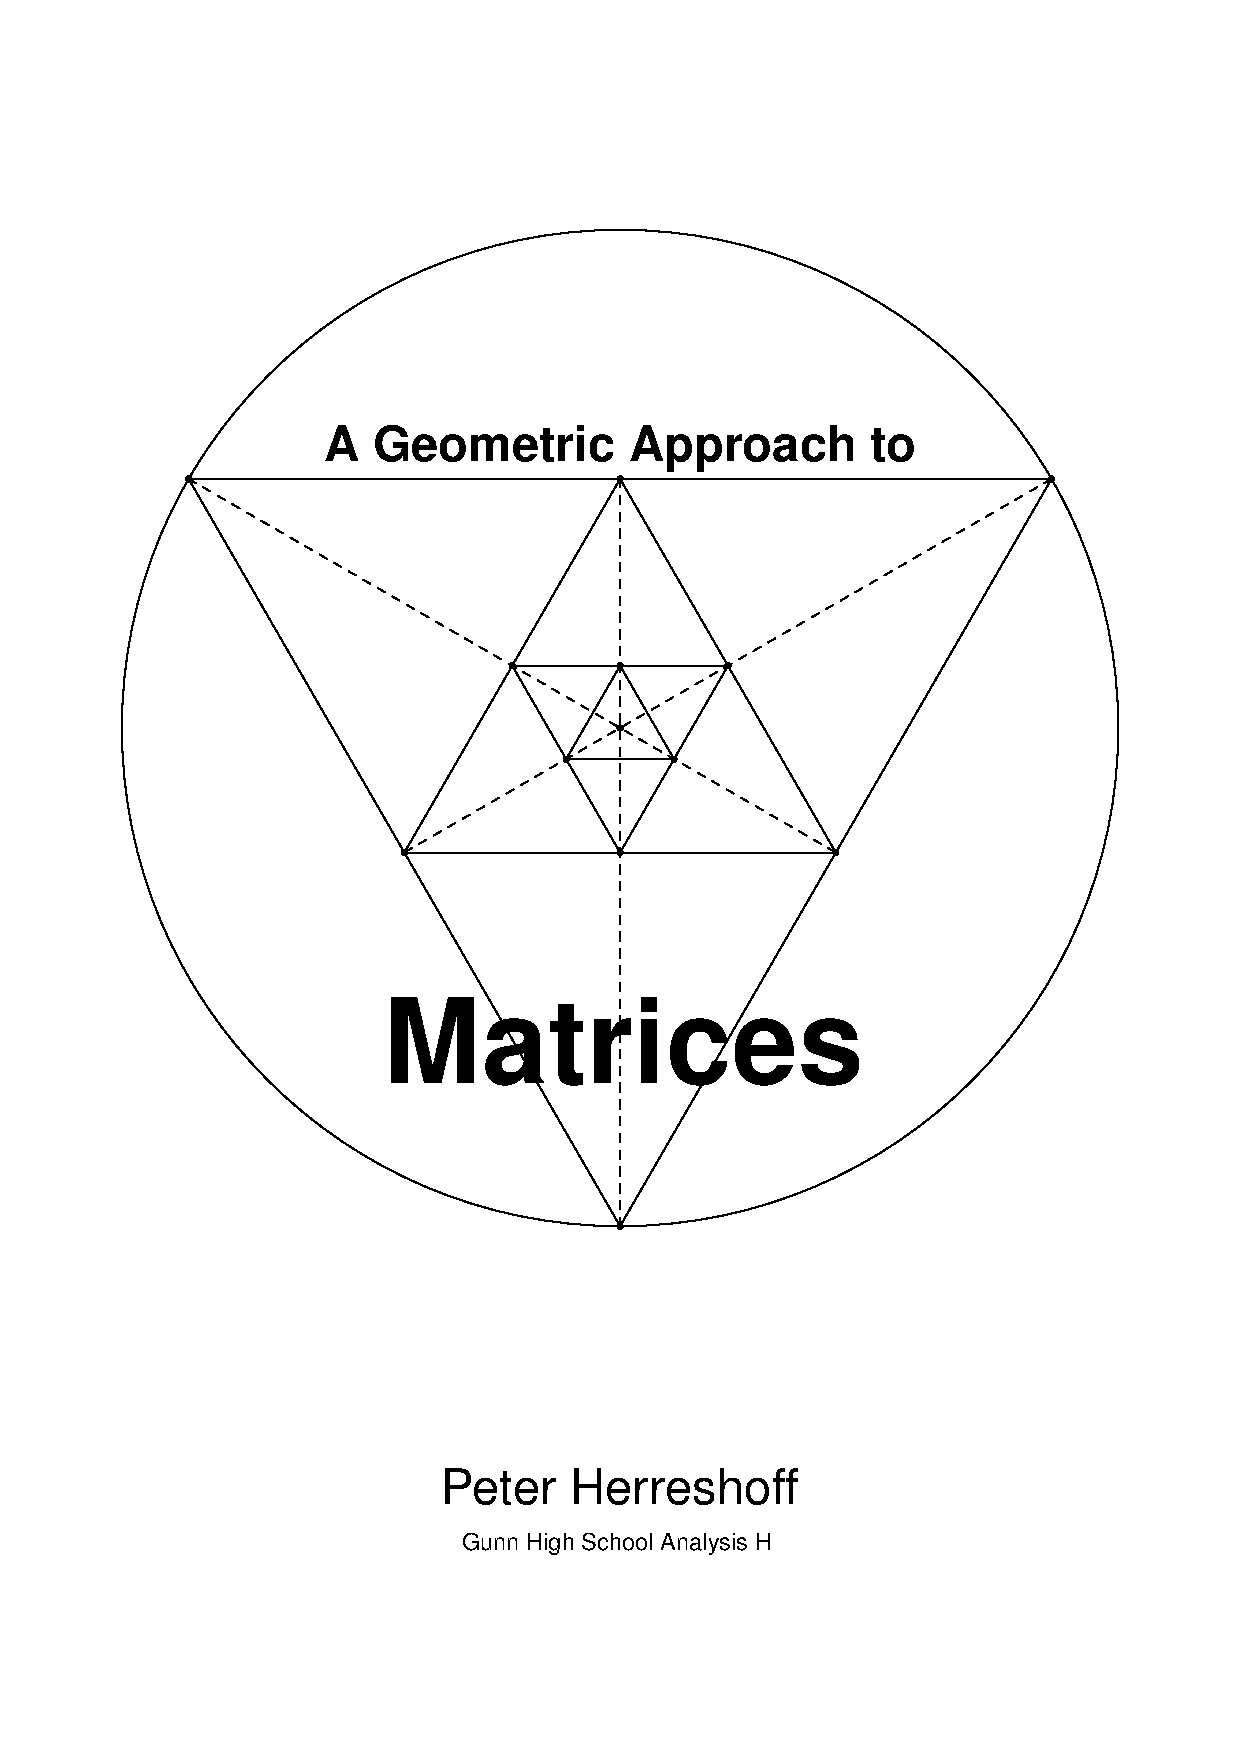
\includepdf[noautoscale=true,pages=-,width=\paperwidth]{./cover/cover_source.pdf} % cover

\subfile{credits/credits_source.tex}
\setcounter{page}{0}
\pagebreak
\pagenumbering{arabic}

% Reset to correct value
\setlength{\parskip}{0em}

\restoregeometry % Because the credits have a different margin setting

\setlength{\parskip}{0.5em}

\tableofcontents
\pagebreak

\subfile{itsasnap/itsasnap_source.tex}
\pagebreak

\subfile{fromsnapstoflips/fromsnapstoflips_source.tex}
\pagebreak

\subfile{rrg/rrg_source.tex} % Rotation reflection groups
\pagebreak

\subfile{inf/inf_source.tex} % Infinite groups
\pagebreak

\subfile{cmplx_geo/cmplx_geo_source.tex} % Geometry of complex numbers
\pagebreak

\subfile{vitamin_i/vitamin_i_source.tex} % Vitamin i
\pagebreak

\subfile{mtrx_mult/mtrx_mult_source.tex} % Matrix multiplication

\end{document}